\subsubsection{CentralServer}

\textbf{Ansvar}\\
\gls{CS} har til ansvar at få videreformidlet kommandoer og fungerer på denne måde som mellemled imellem pakkerne. Derudover har \gls{CS} også ansvar for at indsætte og hente data fra databasen.\\

\textbf{Sekvensdiagram}

\begin{figure}[H]
    \centering
    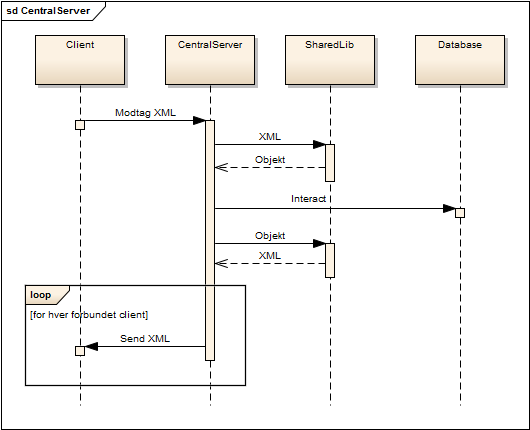
\includegraphics[width=0.8\textwidth]{Systemarkitektur/LogiskView/CentralServer.PNG}
    \caption{Sekvensdiagram for kommunikationen mellem \gls{CS} og andre pakker.}
    \label{fig:cssekv}
\end{figure}

På figur \ref{fig:cssekv} ses hvordan \gls{CS}, når den modtager XML, benytter \gls{SL} til at konvertere det modtagede XML til et højniveau kommando objekt, som \gls{CS} herefter kan agere på. Det enten værende indsættelse/sletning af data i databasen eller andet. Til sidst vil \gls{CS} igen benytte \gls{SL} til at konverete et højniveau svar om til XML, som sendes ud til alle tilstedeværende klienter.\\\\

Dette er den typiske sekvens af kommunikation mellem klient og server, men det er ikke noget krav, at \gls{CS} agerer på den modtagede besked, eller for den sags skyld svarer tilbage til klienten.